\begin{frame}
  \frametitle{\mcmt: Model-Checking Modulo Theories}

  \mcmt is a Model-Checker invented and developed by S. Ghilardi and S. Ranise et al.
  (see http://www.dsi.unimi.it/~ghilardi/mcmt/ for complete and precise 
   acknowledgements) 
  \vfill
  It implements a Symbolic Backward-Reachability algorithm (it relies on yices)
  \vfill
  It was invented to handle safety properties for 
  distributed algorithms (protocols), which
  are infinite-state systems
   
\end{frame}

\subsection{Two simple protocols}

\begin{frame}
  \frametitle{\mcmt demo}
  The following example is taken from the tutorial 
  \vfill
  \begin{center}
  Model Checking Modulo Theories: Theory and Practice
  \end{center}
  \vfill
  available at \url{http://st.fbk.eu/MCMTtutorial}
\end{frame}

\begin{frame}
  \frametitle{A simple protocol}
  \framesubtitle{Description}

  \begin{columns}
  \begin{column}{0.3\textwidth}
    \centering
    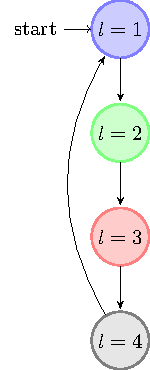
\includegraphics{pictures/demo-prot1-fig}
  \end{column}

  \begin{column}{0.7\textwidth}
    \begin{itemize}
      \item No data, only locations

      \item All processes start from the $1^{\text{st}}$ location

      \item A process in location $3$ is inside the critical section

      \item We want to check if the protocol ensures the mutual exclusion,
	    i.e., at most one process is inside the critical section

    \end{itemize}
  \end{column}

  \end{columns}  

\end{frame}

\begin{frame}[fragile]
  \frametitle{A simple protocol}
  \framesubtitle{Variable}

\begin{columns}
\begin{column}{0.3\textwidth}
\centering
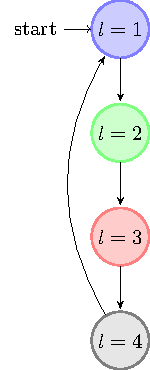
\includegraphics{pictures/demo-prot1-fig}
\end{column}

\begin{column}{0.7\textwidth}
  \begin{itemize}
    \item One {\it local} variable {\tt l}
  \end{itemize}
{\small  
  \begin{verbatim}
  :smt (define-type locations (subrange 1 4))

  :local l locations
  \end{verbatim}
}
\end{column}

\end{columns}  

\end{frame}

\begin{frame}[fragile]
  \frametitle{A simple protocol}
  \framesubtitle{Initial configuration}

  \begin{columns}
  \begin{column}{0.3\textwidth}
  \centering
  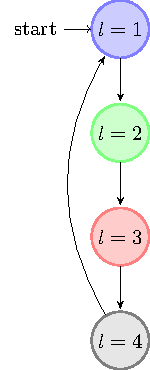
\includegraphics{pictures/demo-prot1-fig}
  \end{column}
  \begin{column}{0.7\textwidth}
  
  \begin{itemize}
    \item All processes start in location $1$
  \end{itemize}

  $$
  \forall x. ({\tt l}[x] = 1)
  $$

  \pause

  \begin{verbatim}
  :initial
  :var x
  :cnj (= l[x] 1)
  \end{verbatim}
  \end{column}

  \end{columns}  

\end{frame}

\begin{frame}[fragile]
  \frametitle{A simple protocol}
  \framesubtitle{Unsafe configuration}

  \begin{columns}
  \begin{column}{0.3\textwidth}
  \centering
  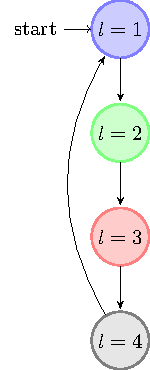
\includegraphics{pictures/demo-prot1-fig}
  \end{column}
  \begin{column}{0.7\textwidth}
  
  \begin{itemize}
    \item Mutual exclusion: At most one process is in location $3$
  \end{itemize}

\pause

\only<1|handout:0>{
$$
U:=\neg\forall z_1, z_2. \left( \left( {\tt l}[z_1] = 3 \wedge {\tt l}[z_2] = 3 \right) \Rightarrow z_1 = z_2 \right)
$$
}
\only<2->{
$$
U:=\exists z_1, z_2. \left( {\tt l}[z_1] = 3 \wedge  {\tt l}[z_2] = 3 \wedge z_1 \neq z_2 \right)
$$
}

\pause
  
  \begin{verbatim}
  :unsafe
  :var z1
  :var z2
  :cnj (= l[z1] 3) (= l[z2] 3)
  \end{verbatim}
\end{column}

\end{columns}  

\end{frame}

\begin{frame}[fragile]
  \frametitle{A simple protocol}
  \framesubtitle{Transitions}

  \begin{columns}
  \begin{column}{0.3\textwidth}
  \centering
  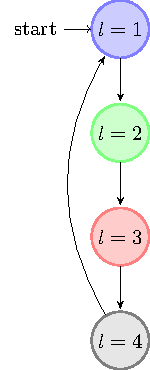
\includegraphics{pictures/demo-prot1-fig}
  \end{column}
  \begin{column}{0.7\textwidth}
  
  \begin{itemize}
    \item A process in location $1$ moves to location $2$
  \end{itemize}

  \vspace{-0.5cm}

  $$
  \tau_1:= \exists x. \left(
  \begin{aligned}
  & {\tt l}[x] = 1 ~\wedge\\
  & {\tt l}' = \lambda j. \left({\sf if}~(x = j)~{\sf then}~2~{\sf else}~{\tt l}[j]\right)
  \end{aligned}
  \right)
  $$
  \pause
 {\footnotesize 
  \begin{verbatim}
  :transition
  :var x
  :var j
  :guard (= l[x] 1)
  :numcases 2
  :case (= x j)
   :val 2
  :case (not (= x j))
   :val l[j]
  \end{verbatim}
 }
\end{column}

\end{columns}  

\end{frame}

\begin{frame}[fragile]
  \frametitle{A simple protocol}
  \framesubtitle{Transitions}

  \begin{columns}
  \begin{column}{0.3\textwidth}
  \centering
  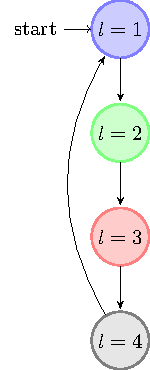
\includegraphics{pictures/demo-prot1-fig}
  \end{column}
  \begin{column}{0.7\textwidth}
  
\begin{columns}
\begin{column}{0.35\textwidth}
 {\scriptsize 
  \begin{verbatim}
  :transition
  :var x
  :var j
  :guard (= l[x] 1)
  :numcases 2
  :case (= x j)
   :val 2
  :case (not (= x j))
   :val l[j]

  :transition
  :var x
  :var j
  :guard (= l[x] 3)
  :numcases 2
  :case (= x j)
   :val 4
  :case (not (= x j))
   :val l[j]
 \end{verbatim}
 }
\end{column}
\begin{column}{0.35\textwidth}
 {\scriptsize 
  \begin{verbatim}
  :transition
  :var x
  :var j
  :guard (= l[x] 2)
  :numcases 2
  :case (= x j)
   :val 3
  :case (not (= x j))
   :val l[j]
  
  :transition
  :var x
  :var j
  :guard (= l[x] 4)
  :numcases 2
  :case (= x j)
   :val 1
  :case (not (= x j))
   :val l[j]
 \end{verbatim}
 }
\end{column}

\end{columns}  

\end{column}

\end{columns}

\end{frame}

\begin{frame}[fragile]
  \frametitle{A simple protocol}
  \framesubtitle{Execution}

  \begin{columns}
  \begin{column}{0.3\textwidth}
  \centering
  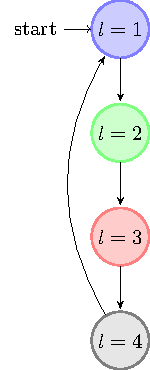
\includegraphics{pictures/demo-prot1-fig}
  \end{column}
  \begin{column}{0.7\textwidth}
  
  \begin{itemize}
    \item {\tt \$ ./mcmt simple\_unsafe.in}
  \end{itemize}

\end{column}

\end{columns}  

\end{frame}




\begin{frame}[fragile]
  \frametitle{A simple protocol}
  \framesubtitle{Execution - Get informations from counterexample}

{\scriptsize
\begin{verbatim}
[...]
Doing state space exploration...
 node 1= [t2_1][0]  
 node 2= [t1_1][t2_1][0]  
 node 3= [t2_2][t2_1][0]  
 node 4= [t2_2][t1_1][t2_1][0]  
 node 5= [t4_1][t1_1][t2_1][0]  
 node 6= [t1_2][t2_2][t1_1][t2_1][0]

=============================================================================
System is UNSAFE!
[...]
\end{verbatim}
}

\end{frame}




\begin{frame}[fragile]
  \frametitle{A simple protocol}
  \framesubtitle{Counterexample analysis from trace}

\begin{tabular}{rl}
Initial state: & $\forall i.\ (\ {\tt l}[i] = 1\ )$ \\
 Unsafe state: & $\exists {\tt z1}, {\tt z2}.\ (\ {\tt l[z1]}=3 \wedge {\tt l[z2]}=3\ )$ \\
 Counter-example: & \verb|node 6 = |\color<9,10>{red}{\verb|[t1_2]|}\color<7,8>{red}{\verb|[t2_2]|}\color<5,6>{red}{\verb|[t1_1]|}\color<3,4>{red}{\verb|[t2_1]|}\color<2>{red}{\verb|[0]|} 
\end{tabular}

\vfill

\only<1,2|handout:0>{ 
\textcolor{white}{
$$
\tau_2:= \exists x. \left(
\begin{aligned}
& {\tt l}[x] = 2 ~\wedge\\
& {\tt l}' = \lambda j. \left({\sf if}~(x = j)~{\sf then}~3~{\sf else}~{\tt l}[j]\right)
\end{aligned}
\right)
$$
}}
\only<3-4,7-8|handout:0>{ 
$$
\tau_2:= \exists x. \left(
\begin{aligned}
& {\tt l}[x] = 2 ~\wedge\\
& {\tt l}' = \lambda j. \left({\sf if}~(x = j)~{\sf then}~3~{\sf else}~{\tt l}[j]\right)
\end{aligned}
\right)
$$
}
\only<5-6,9-10>{ 
$$
\tau_1:= \exists x. \left(
\begin{aligned}
& {\tt l}[x] = 1 ~\wedge\\
& {\tt l}' = \lambda j. \left({\sf if}~(x = j)~{\sf then}~2~{\sf else}~{\tt l}[j]\right)
\end{aligned}
\right)
$$
}

\vfill

\pause

\begin{tabular}{r|l}

\begin{minipage}{.3\textwidth}
\begin{overlayarea}{\textwidth}{3cm}
\only<2,3|handout:0>{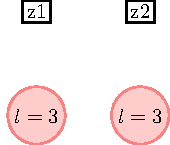
\includegraphics{pictures/demo-prot1-cex-1-fig}}
\only<4,5|handout:0>{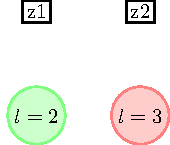
\includegraphics{pictures/demo-prot1-cex-2-fig}}
\only<6,7|handout:0>{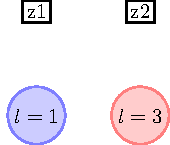
\includegraphics{pictures/demo-prot1-cex-3-fig}}
\only<8,9|handout:0>{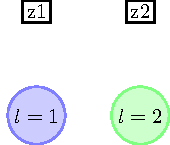
\includegraphics{pictures/demo-prot1-cex-4-fig}}
\only<10>{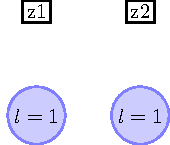
\includegraphics{pictures/demo-prot1-cex-5-fig}}
\end{overlayarea}
\end{minipage}

&

\begin{minipage}{.7\textwidth}
\begin{tabular}{rcl}
     \verb|[0]| & & $\exists {\tt z1}, {\tt z2}.\ (\ {\tt l[z1]}=3 \wedge {\tt l[z2]}=3\ )$ \\
 \pause
 \pause
 \verb|[t2_1]| & & $\exists {\tt z1}, {\tt z2}.\ (\ {\tt l[z1]}=2 \wedge {\tt l[z2]}=3\ )$ \\
 \pause
 \pause
 \verb|[t1_1]| & & $\exists {\tt z1}, {\tt z2}.\ (\ {\tt l[z1]}=1 \wedge {\tt l[z2]}=3\ )$ \\
 \pause
 \pause
 \verb|[t2_2]| & & $\exists {\tt z1}, {\tt z2}.\ (\ {\tt l[z1]}=1 \wedge {\tt l[z2]}=2\ )$ \\
 \pause
 \pause
 \verb|[t1_2]| & & $\exists {\tt z1}, {\tt z2}.\ (\ {\tt l[z1]}=1 \wedge {\tt l[z2]}=1\ )$
\end{tabular}
\end{minipage}

\end{tabular}

\end{frame}




\begin{frame}
  \frametitle{Another simple protocol}
  \framesubtitle{Description}

\begin{columns}
\begin{column}{0.3\textwidth}
\centering
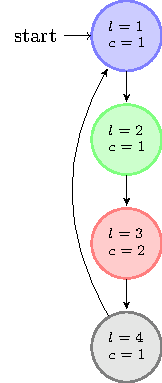
\includegraphics{pictures/demo-prot2-fig}
\end{column}


\begin{column}{0.7\textwidth}
  \begin{itemize}
    \item Like before, but with a \hl{global} flag {\tt c} that
          takes care of mutual exclusion

    \item All processes start from the $1^{\text{st}}$ location

    \item A process in location $3$ is inside the critical section

    \item We want to check if the protocol ensures the mutual exclusion,
	  i.e., at most one process is inside the critical section
  \end{itemize}
\end{column}

\end{columns}  

\end{frame}




\begin{frame}[fragile]
  \frametitle{Another simple protocol}
  \framesubtitle{Variable(s)}

\begin{columns}
\begin{column}{0.3\textwidth}
\centering
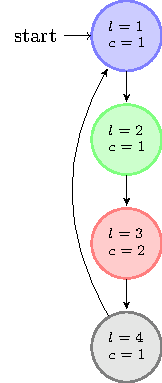
\includegraphics{pictures/demo-prot2-fig}
\end{column}


\begin{column}{0.7\textwidth}
  \begin{itemize}
    \item One {\it local} variable {\tt l}
  \end{itemize}
{\small  
  \begin{verbatim}
  :smt (define-type locations (subrange 1 4))
  :smt (define-type counter (subrange 1 2))

  :local l location
  :global c counter
  \end{verbatim}
}
\end{column}

\end{columns}  

\end{frame}




\begin{frame}[fragile]
  \frametitle{Another simple protocol}
  \framesubtitle{Initial configuration}

\begin{columns}
\begin{column}{0.3\textwidth}
\centering
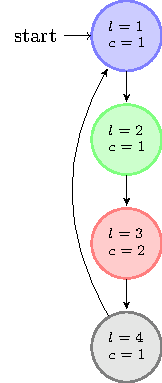
\includegraphics{pictures/demo-prot2-fig}
\end{column}
\begin{column}{0.7\textwidth}
  
  \begin{itemize}
    \item All processes start in location $1$, with counter set to $1$
  \end{itemize}

$$
\forall x.\ (\ {\tt l}[x] = 1 \wedge {\tt c}[x] = 1\ ) 
$$

\pause

  \begin{verbatim}
  :initial
  :var x
  :cnj (= l[x] 1) (= c[x] 1)
  \end{verbatim}
\end{column}

\end{columns}  

\end{frame}



\begin{frame}[fragile]
  \frametitle{Another simple protocol}
  \framesubtitle{Unsafe configuration}

\begin{columns}
\begin{column}{0.3\textwidth}
\centering
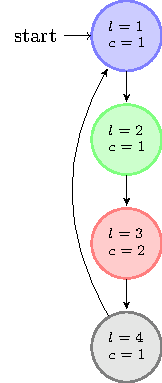
\includegraphics{pictures/demo-prot2-fig}
\end{column}
\begin{column}{0.7\textwidth}
  
  \begin{itemize}
    \item Mutual exclusion: At most one process is in location $3$
  \end{itemize}

\pause

\only<1|handout:0>{
$$
U:=\neg\forall z_1, z_2. \left( \left( {\tt l}[z_1] = 3 \wedge {\tt l}[z_2] = 3 \right) \Rightarrow z_1 = z_2 \right)
$$
}
\only<2->{
$$
U:=\exists z_1, z_2. \left( {\tt l}[z_1] = 3 \wedge  {\tt l}[z_2] = 3 \wedge z_1 \neq z_2 \right)
$$
}

\pause
  
  \begin{verbatim}
  :unsafe
  :var z1
  :var z2
  :cnj (= l[z1] 3) (= l[z2] 3)
  \end{verbatim}
\end{column}

\end{columns}  

\end{frame}





\begin{frame}[fragile]
  \frametitle{Another simple protocol}
  \framesubtitle{Transitions}

\begin{columns}
\begin{column}{0.3\textwidth}
\centering
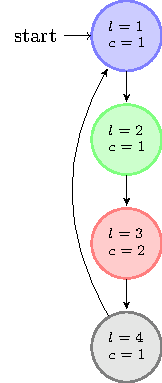
\includegraphics{pictures/demo-prot2-fig}
\end{column}
\begin{column}{0.7\textwidth}
  
%  \begin{itemize}
%    \item A process in location $2$, can move to location $3$ only if $c = 1$.
%  \end{itemize}

%\vspace{-0.5cm}

{\footnotesize
$$
\tau_2:= \exists x. \left(
\begin{aligned}
& {\tt l}[x] = 2 \wedge {\tt c}[x] = 1\ \wedge \\
& {\tt l}' = \lambda j. \left({\sf if}~(x = j)~{\sf then}~3~{\sf else}~{\tt l}[j]\right) \\
& {\tt c}' = \lambda j. 2
\end{aligned}
\right)
$$
}

\vspace{-14pt}

\pause
 {\footnotesize 
  \begin{verbatim}
  :transition
  :var x
  :var j
  :guard (= l[x] 2) (= c[x] 1)
  :numcases 2
  :case (= x j)
   :val 3
   :val 2
  :case (not (= x j))
   :val l[j]
   :val 2
  \end{verbatim}
 }
\end{column}

\end{columns}  

\end{frame}





\begin{frame}[fragile]
  \frametitle{Another simple protocol}
  \framesubtitle{Transitions}

\begin{columns}
\begin{column}{0.3\textwidth}
\centering
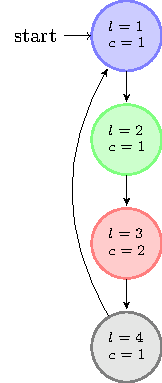
\includegraphics{pictures/demo-prot2-fig}
\end{column}
\begin{column}{0.7\textwidth}
  
\begin{columns}
\begin{column}{0.35\textwidth}
 {\tiny 
  \begin{verbatim}
  :transition
  :var x
  :var j
  :guard (= l[x] 1) 
  :numcases 2
  :case (= x j)
   :val 2
   :val c[x]
  :case (not (= x j))
   :val l[j]
   :val c[x]

  :transition
  :var x
  :var j
  :guard (= l[x] 3) (= c[x] 2)
  :numcases 2
  :case (= x j)
   :val 4
   :val 1
  :case (not (= x j))
   :val l[j]
   :val 1
 \end{verbatim}
 }
\end{column}
\begin{column}{0.35\textwidth}
 {\tiny 
  \begin{verbatim}
  :transition
  :var x
  :var j
  :guard (= l[x] 2) (= c[x] 1)
  :numcases 2
  :case (= x j)
   :val 3
   :val 2
  :case (not (= x j))
   :val l[j]
   :val 2
  
  :transition
  :var x
  :var j
  :guard (= l[x] 4) 
  :numcases 2
  :case (= x j)
   :val 1
   :val c[j]
  :case (not (= x j))
   :val l[j]
   :val c[j]
 \end{verbatim}
 }
\end{column}

\end{columns}  

\end{column}

\end{columns}

\end{frame}






\begin{frame}[fragile]
  \frametitle{Another simple protocol}
  \framesubtitle{Execution}

\begin{columns}
\begin{column}{0.3\textwidth}
\centering
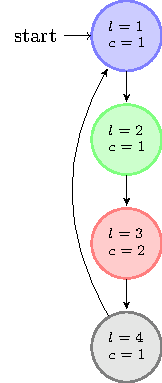
\includegraphics{pictures/demo-prot2-fig}
\end{column}
\begin{column}{0.7\textwidth}
  
  \begin{itemize}
    \item {\tt \$ ./mcmt simple\_safe.in}
  \end{itemize}

\end{column}

\end{columns}  

\end{frame}




\begin{frame}[fragile]
  \frametitle{Another simple protocol}
  \framesubtitle{Execution}

{\scriptsize
\begin{verbatim}
[...]
Doing state space exploration...
 node 1 = [t2_1][0]  
 node 2 = [t1_1][t2_1][0]  
 node 3 = [t4_1][t1_1][t2_1][0]  

=============================================================================
Global fixpoint reached!

System is SAFE!
[...]
\end{verbatim}
}

\end{frame}




\begin{frame}[fragile]
  \frametitle{A simple protocol}
  \framesubtitle{Set of (un)reachable states}

\begin{tabular}{rl}
Initial state: & $\forall i.\ (\ {\tt l}[i] = 1 \wedge {\tt c}[i] = 1\ )$ \\
 Unsafe state: & $\exists {\tt z1}, {\tt z2}.\ (\ {\tt l[z1]}=3 \wedge {\tt l[z2]}=3\ )$ \\
\end{tabular}

\vfill

\begin{columns}

\begin{column}{.3\textwidth}
\begin{overlayarea}{\textwidth}{7cm}
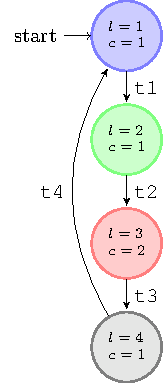
\includegraphics[scale=.8]{pictures/demo-prot2-s-fig}
\end{overlayarea}
\end{column}

\begin{column}{.18\textwidth}
\begin{overlayarea}{\textwidth}{8cm}
\only<1|handout:0>{\vspace{150pt}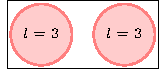
\includegraphics[scale=.6]{pictures/demo-prot2-s-1-fig}}
\only<2|handout:0>{\vspace{113pt}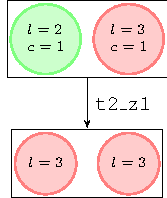
\includegraphics[scale=.6]{pictures/demo-prot2-s-2-fig}}
\only<3|handout:0>{\vspace{77pt}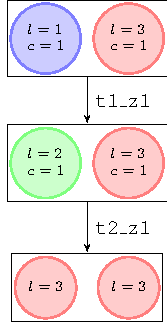
\includegraphics[scale=.6]{pictures/demo-prot2-s-3-fig}}
\only<4|handout:0>{\vspace{41pt}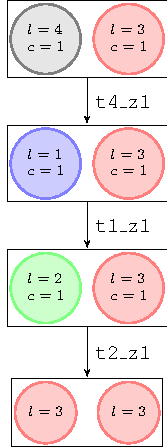
\includegraphics[scale=.6]{pictures/demo-prot2-s-4-fig}}
\only<5|handout:0>{\vspace{5pt}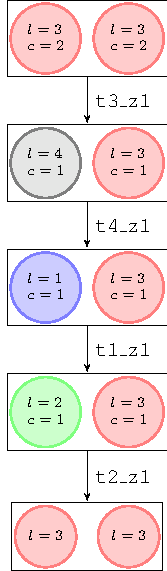
\includegraphics[scale=.6]{pictures/demo-prot2-s-5-fig}}
\only<6>{\vspace{41pt}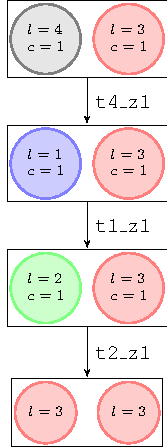
\includegraphics[scale=.6]{pictures/demo-prot2-s-4-fig}}
\end{overlayarea}
\end{column}

\begin{column}{.52\textwidth}
\vspace{-1cm}
{\scriptsize
$$
\tau_1 := \exists x. \left(
\begin{aligned}
& {\tt l}[x] = 1 \ \wedge \\
& {\tt l}' = \lambda j. \left({\sf if}~(x = j)~{\sf then}~2~{\sf else}~{\tt l}[j]\right) \\
& {\tt c}' = \lambda j. {\tt c}[j]
\end{aligned}
\right)
$$
$$
\tau_2 := \exists x. \left(
\begin{aligned}
& {\tt l}[x] = 2 \wedge {\tt c}[x] = 1\ \wedge \\
& {\tt l}' = \lambda j. \left({\sf if}~(x = j)~{\sf then}~3~{\sf else}~{\tt l}[j]\right) \\
& {\tt c}' = \lambda j. 2
\end{aligned}
\right)
$$
$$
\tau_3 := \exists x. \left(
\begin{aligned}
& {\tt l}[x] = 3 \wedge {\tt c}[x] = 2\ \wedge \\
& {\tt l}' = \lambda j. \left({\sf if}~(x = j)~{\sf then}~4~{\sf else}~{\tt l}[j]\right) \\
& {\tt c}' = \lambda j. 1
\end{aligned}
\right)
$$
$$
\tau_4 := \exists x. \left(
\begin{aligned}
& {\tt l}[x] = 4 \ \wedge \\
& {\tt l}' = \lambda j. \left({\sf if}~(x = j)~{\sf then}~1~{\sf else}~{\tt l}[j]\right) \\
& {\tt c}' = \lambda j. {\tt c}[j]
\end{aligned}
\right)
$$
}
\end{column}

\end{columns}

\end{frame}
